The implementation supports three distinct initial conditions for the scalar field and its canonical momentum. These include a plane wave, an exact Gaussian, and a multipolar Gaussian function. The plane wave and exact Gaussian initial data were developed for the purpose of testing the projections of derivative operators detailed in Sec.\ref{ch:wave_scattering:sec:multipatch}. The exact Gaussian initial data is named as such to reflect the fact that it is an exact solution of the Klein-Gordon equation in flat spacetime.

The process of computing the derivative projection tests was carried out in the following manner: Prior to executing a time evolution step of the system, the right-hand side (RHS) of the evolution system was calculated using the initial data and subsequently stored. Due to the known and simple nature of the initial data, it is feasible to determine the RHS separately from the \texttt{Thorn} and validate its accuracy by performing a direct comparison. If the discrepancy between the results provided by the \texttt{Thorn} and those computed independently was within the range of floating point precision, the test was deemed to have been successful.

\subsection{Plane wave initial data}

The plane wave solution is given by
%
\begin{equation}
  P_w(t,x,y,z) = \cos\omega
\end{equation}
%
where the auxiliary variables are defined as
\begin{align}
  \Omega & = \sqrt{K_x^2 + K_y^2 + K_z^2}               \\
  n_t    & = \Omega * (t - t_0)                         \\
  n_x    & = K_x * (x - x_0)                            \\
  n_y    & = K_y * (y - y_0)                            \\
  n_z    & = K_z * (z - z_0)                            \\
  \omega & = 2 \pi \left( n_t + n_x + n_y + n_z \right)
\end{align}
%
and the parameters $K_{x,y,z}$ and $(t,x,y,z)_0$ are real numbers freely specified in the code, representing the wave number and wave offsets, respectively.

Figure \ref{fig:multipolar_plane_wave_id_demo} is a plot of $P_w(t,x,y,z)$ with parameters $K_x = K_y = K_z = 1$ and $t_0 = x_0 = y_0 = z_0 = 0$ at time $t=0$ and $z=0$.

\begin{figure}[!ht]
  \centering
  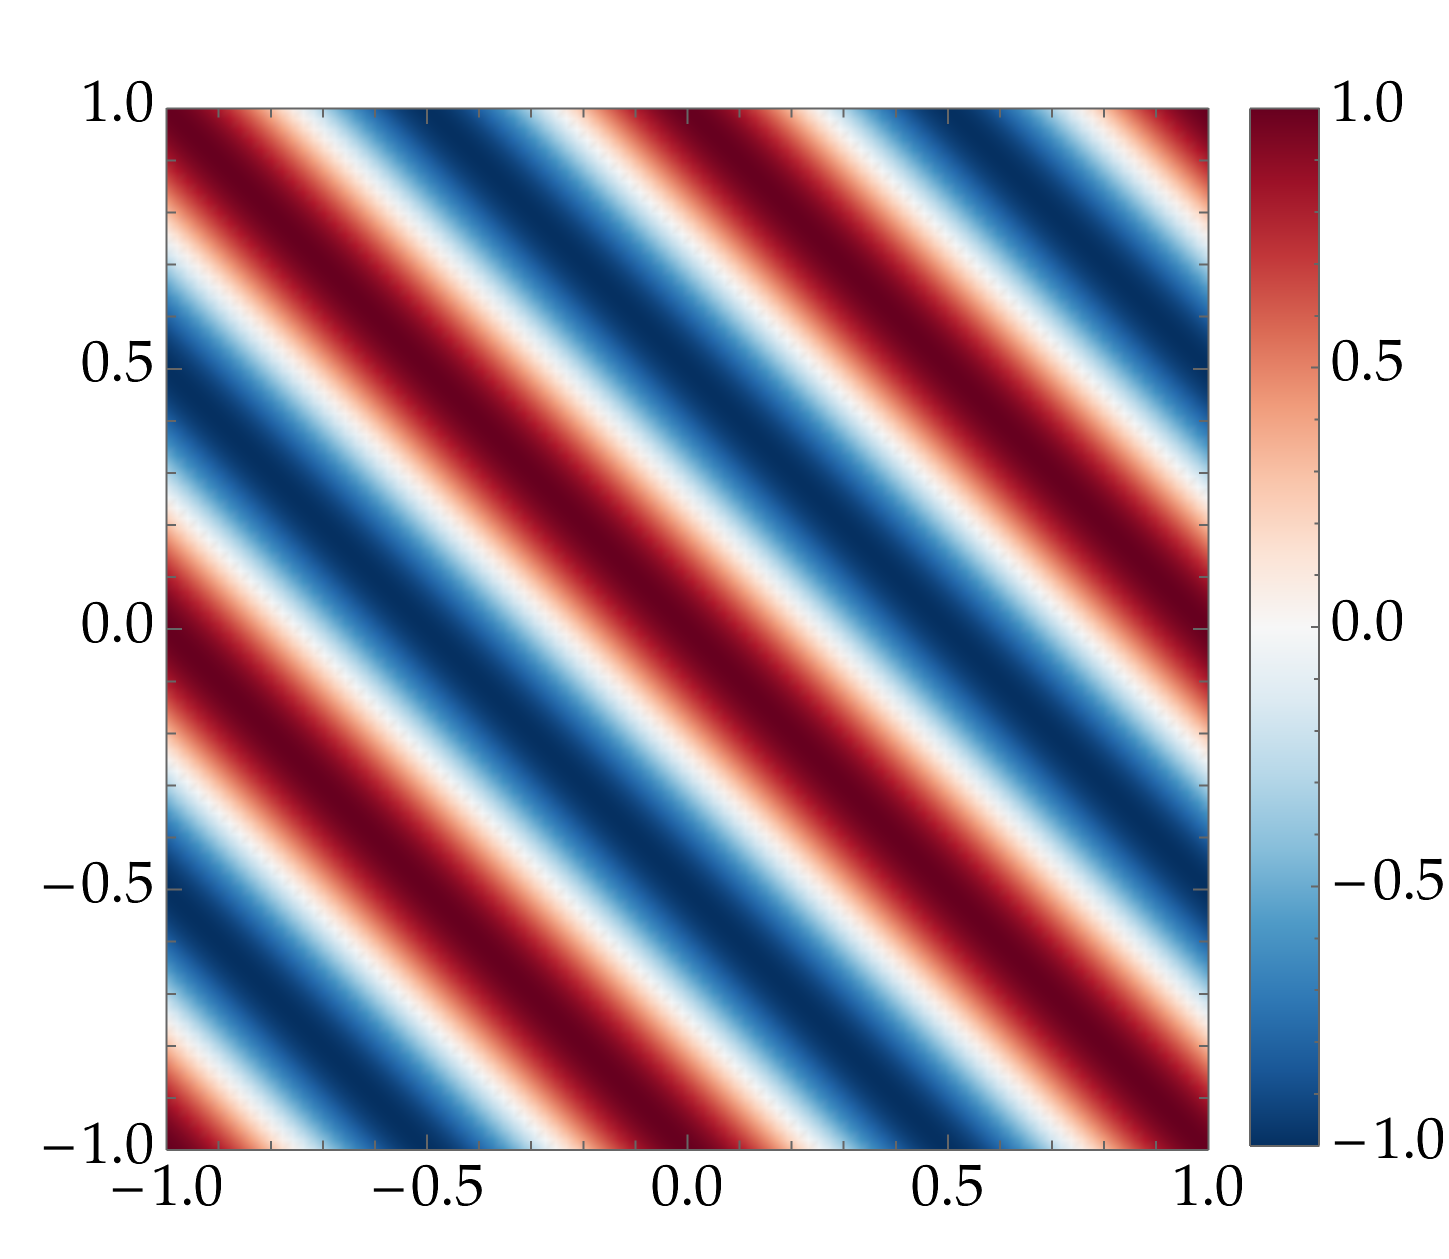
\includegraphics[width=0.5\linewidth]{img/wave_scattering/plane_wave_id_examples.png}
  \caption{Demonstration of the plane wave initial data with parameters $K_x = K_y = Kz = 1$ and $t_0 = x_0 = y_0 = z_0 = 0$ at time $t=0$ and $z=0$.}
  \label{fig:multipolar_plane_wave_id_demo}
\end{figure}

\subsection{Exact Gaussian initial data}

From the basic Gaussian function
%
\begin{equation}
  G(r, \sigma) = \exp\left( -\frac{1}{2} \left( \frac{r}{\sigma} \right)^2  \right),
  \label{eq:wave_scattering_gaussian}
\end{equation}
%
where $\sigma$ represents the Gaussian width and is freely specified in the code, the general solution for the flat spacetime Klein-Gordon equation can then be written as
\begin{equation}
  E_G(t, r, \sigma) = \left( G(r-t, \sigma) - G(r+t, \sigma) \right) / r.
  \label{eq:wave_scattering_exact_gaussian}
\end{equation}

By utilizing the Eq.~\eqref{eq:wave_scattering_exact_gaussian} and its derivatives at $t=0$ as the initial conditions for the evolution system under Minkowski spacetime, one can examine the total error of the evolution by evaluating the difference between Eq.~\eqref{eq:wave_scattering_exact_gaussian} at $t>0$ and the numerically evolved data. Figure \ref{fig:multipolar_exact_gaussian_id_demo} illustrates the initial data at different times.

\begin{figure}[!ht]
  \centering
  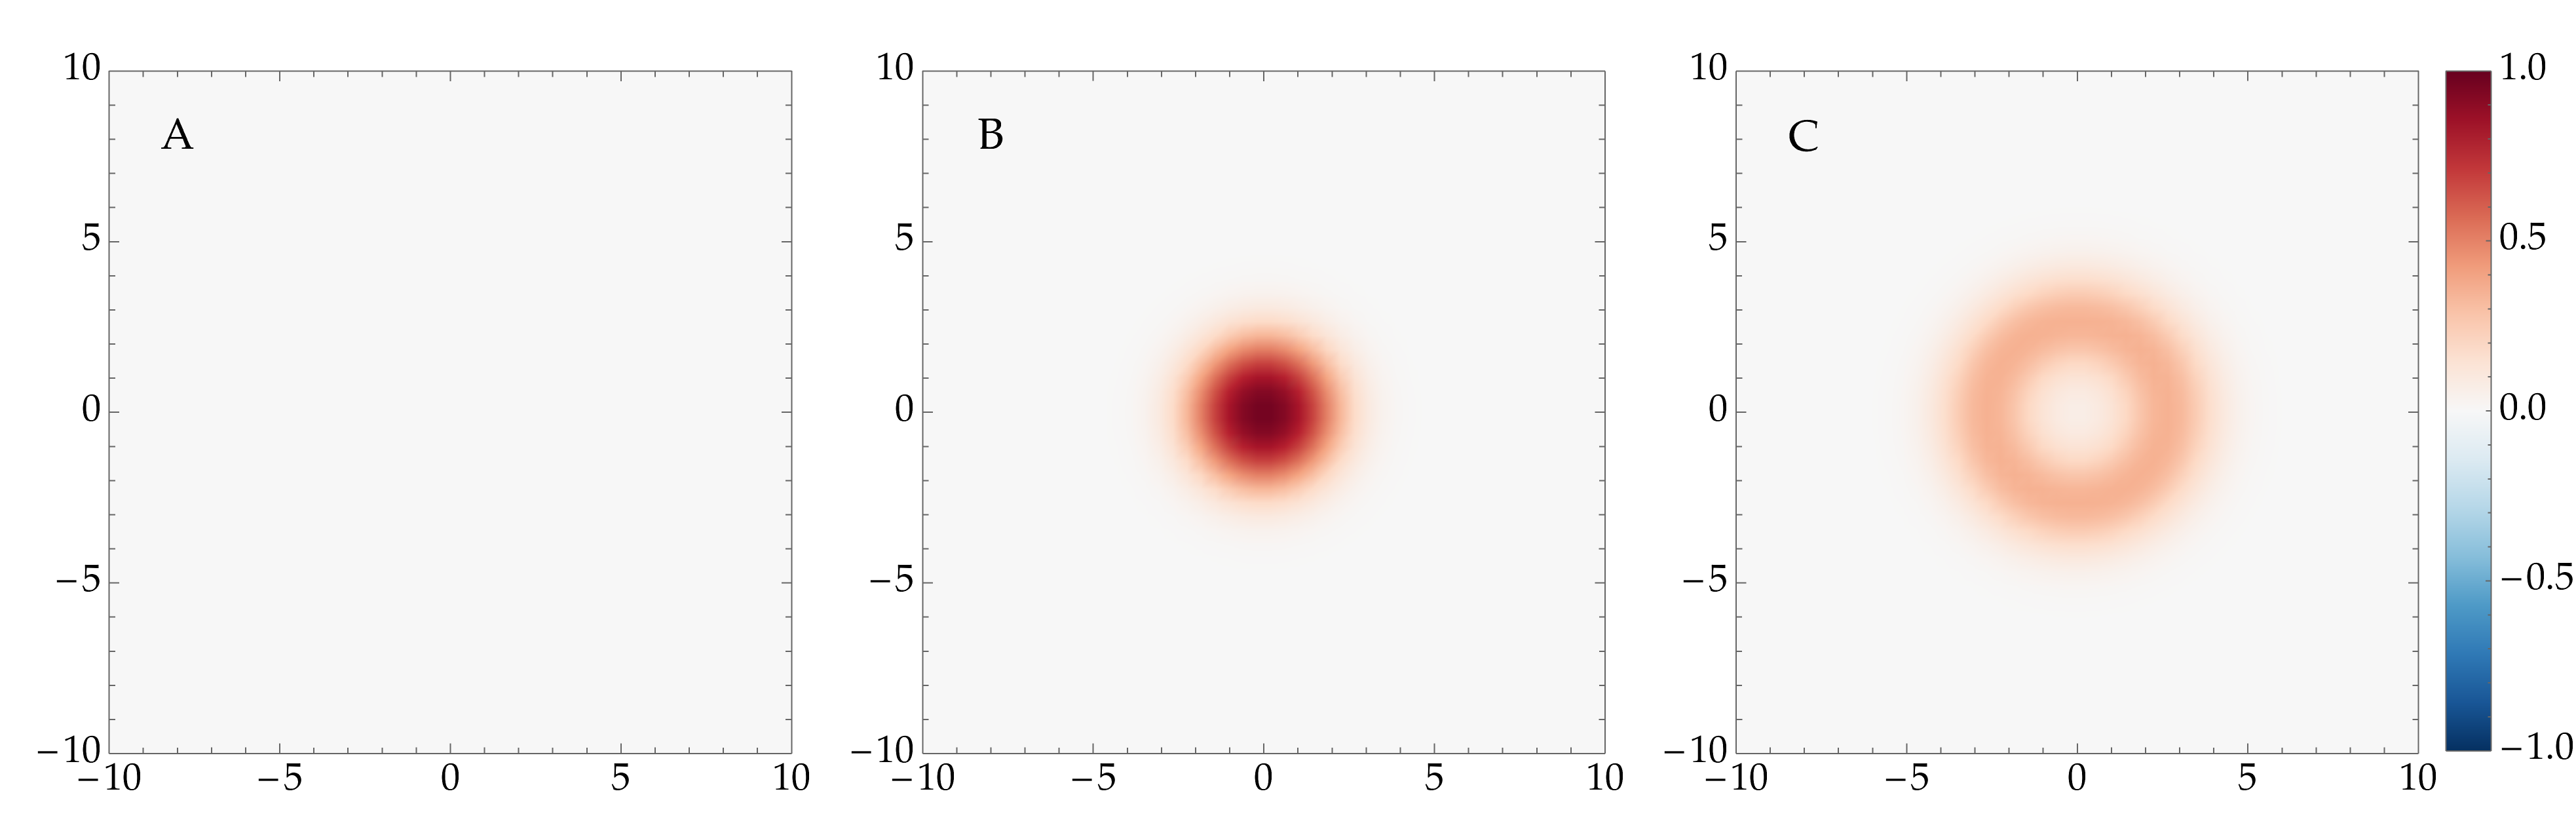
\includegraphics[width=\linewidth]{img/wave_scattering/exact_gaussian_id_examples.png}
  \caption{Demonstration of the multipolar exact Gaussian data at different time intervals. For all panels, $\sigma = 1$. Panel \textbf{A} displays the function at $t=0$, Panel \textbf{B}, at $t = 1.5$, and Panel \textbf{C} at $t=3$.}
  \label{fig:multipolar_exact_gaussian_id_demo}
\end{figure}

\subsection{Multipolar Gaussian initial data}

The multipolar Gaussian function is a basic Gaussian function that is multiplied by a linear combination of real spherical harmonics. This particular function was the one chosen during our production runs\footnote{A production run refers to the execution of a program that is intended to generate results, in contrast to testing runs or benchmarking runs where the purpose is to evaluate the code or measure its performance characteristics.} as it has the ability to excite specific modes in the system based on the chosen parameters for the linear combination.

The development of this initial data is based on the methodology presented in Ref.~\cite{PhysRevD.87.043513}. In order to construct it, let us first introduce its components. We start with the Gaussian function $G(r, \sigma)$ of Eq.~\eqref{eq:wave_scattering_gaussian}. Next, we introduce the real spherical harmonics $Y_{lm}(x,y,z)$, given by
%
\begin{equation}
  Y_{lm}(x, y, z) =
  \begin{cases}
    A_{lm} P_{lm}\left( \frac{z}{\sqrt{x^2 + y^2 + z^2}} \right) \cos(m \arctan(y,x)) \text{ if } m \geq 0  \\
    A_{lm} P_{l|m|}\left( \frac{z}{\sqrt{x^2 + y^2 + z^2}} \right) \sin(|m| \arctan(y,x)) \text{ if } m < 0 \\
  \end{cases}
  ,
  \label{eq:wave_scattering_real_spherical_harmonics}
\end{equation}
%
where $P_{lm}(x)$ are the associated Legendre polynomials and the $A_{lm}$ coefficients are given by
%
\begin{equation}
  A_{lm} = (-1)^m \sqrt{\frac{2 l + 1}{4\pi} \frac{(l-m)!}{(l+m)!}}.
  \label{eq:wave_scattering_real_spherical_harmonics_coeffs}
\end{equation}
%
By introducing
%
\begin{align}
  X & \equiv x - x_0 \label{eq:wave_scattering_real_spherical_harmonics_shifted_x}                \\
  Y & \equiv y - y_0 \label{eq:wave_scattering_real_spherical_harmonics_shifted_y}                \\
  Z & \equiv z - z_0 \label{eq:wave_scattering_real_spherical_harmonics_shifted_z}                \\
  R & \equiv \sqrt{X^2 + Y^2 + Z^2} \label{eq:wave_scattering_real_spherical_harmonics_shifted_r}
\end{align}
%
it is possible to shift the location of the center of the function to $(x_0,y_0,z_0)$. Combining these pieces, the multipolar Gaussian function $M_G(x,y,z)$ is written as
%
\begin{equation}
  M_G(x, y, z) = \sum_{l=0}^{N}\sum_{m = -l}^{l} c_{l m} Y_{l m}(X,Y,Z) G(R-R_0,\sigma)
  \label{eq:wave_scattering_multipolar_gaussian}
\end{equation}
%
where $R_0$ is the radius of the Gaussian function and the $c_{l m}$ coefficients are free parameters. Once again, code generation routines for the initial data can be found in \texttt{Notebooks/equation.nb} of Ref.~\cite{FieldPerturbationsRepo}. It is important to note that in the implemented code, the series is expanded up to $N = 2$, and higher multipole orders are not supported.

Figure~\ref{fig:multipolar_gaussian_id_demo} showcases three distinct configurations of the multipolar Gaussian function. For all panels, the parameters $x_0$, $y_0$, and $z_0$ were assigned a value of zero, while $R_0$ was set to 5. Panel \textbf{A} displays a plot where $c_{00}$ is assigned a value of $1/A_{00}$, and all other coefficients are set to zero. In Panel \textbf{B}, $c_{11}$ is set to $1/A_{11}$, and all other coefficients are set to zero. Finally, in Panel \textbf{C}, $c_{22}$ is assigned a value of $1/(3A_{22})$, and all other coefficients are set to zero.

\begin{figure}[!ht]
  \centering
  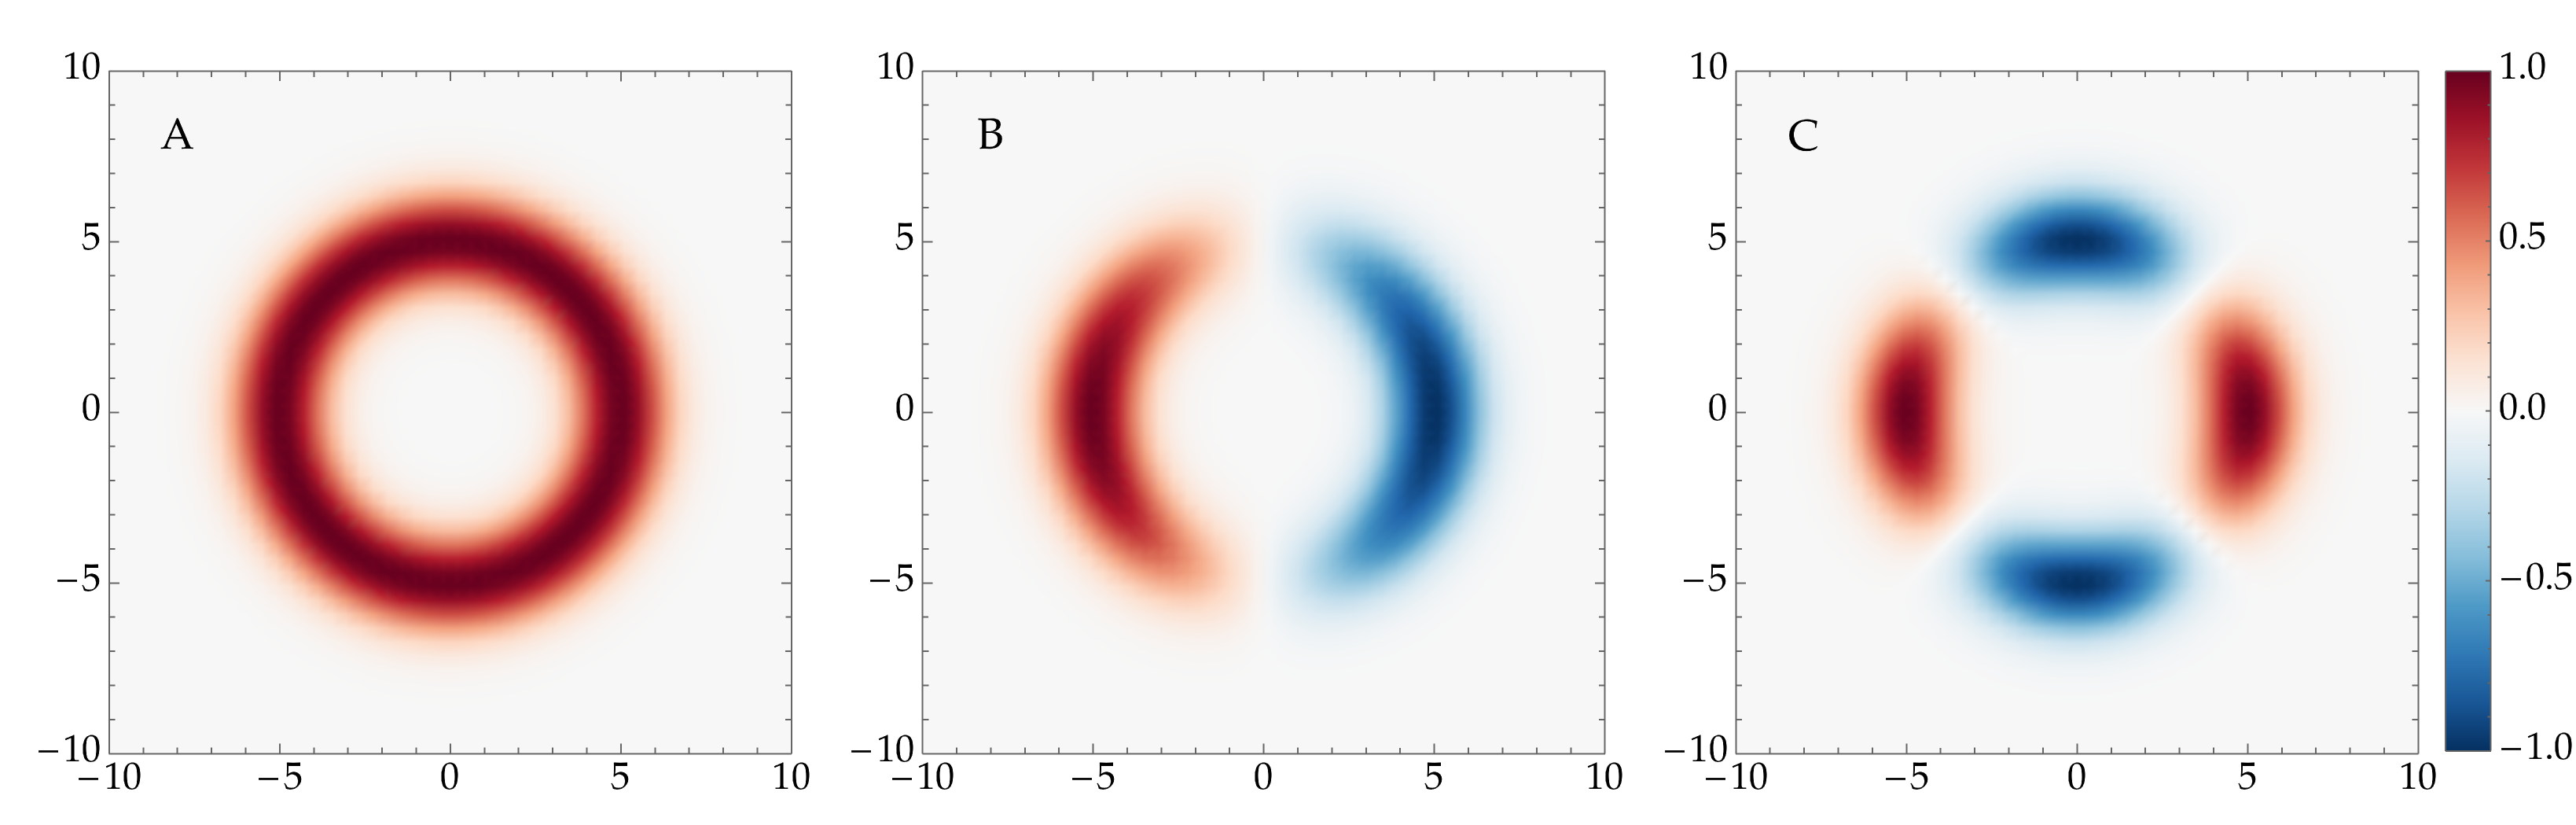
\includegraphics[width=\linewidth]{img/wave_scattering/multipolar_gaussian_id_examples.png}
  \caption{Demonstration of the multipolar Gaussian function with different parameters. For all panels, $x_0 = y_0 = z_0 = 0$ and $R_0 = 5$. In Panel \textbf{A} displays the only nonzero coefficient is $c_{00} = 1/A_{00}$, in Panel \textbf{B}, $c_{11} = 1/A_{11}$, and in Panel \textbf{C}, $c_{22} = 1/(3A_{22})$.}
  \label{fig:multipolar_gaussian_id_demo}
\end{figure}